\documentclass[conference]{IEEEtran}
\IEEEoverridecommandlockouts
% The preceding line is only needed to identify funding in the first footnote. If that is unneeded, please comment it out.
\usepackage{cite}
\usepackage{amsmath,amssymb,amsfonts}
\usepackage{algorithmic}
\usepackage{graphicx}
\usepackage{textcomp}
\usepackage{xcolor}
\usepackage[UTF8]{ctex}

\def\BibTeX{{\rm B\kern-.05em{\sc i\kern-.025em b}\kern-.08em
T\kern-.1667em\lower.7ex\hbox{E}\kern-.125emX}}
\begin{document}

\title{可移动机械臂对物体的搬运——以PUMA560为例}
\author{王柯然\ \ \ \ 2100017727}

\maketitle

\section{引言}
在生活中我们经常会遇到各种类型的机器人,其中很大一部分都是机械臂。机械臂是一种能够模拟人类手臂运动的装置,通常由多个关节组成。一般情况下,机械臂是一端固定的,这导致机械臂可以触及到的范围十分有限。
因此,我们试图考虑可移动的机械臂,在现实中,我们可以把机械臂安装在可移动的小车上以实现这一模型。具有了可移动性,机械臂就可以在工厂、仓库、医院等环境中灵活运用。
在这篇报告中,我们着重考虑机械臂对物体的搬运,机械臂可以用于搬运、装配、堆垛等任务,从而提高生产效率和减轻人力劳动。

这个选题对于许多问题的解决都有意义,具体有如下几种应用场景:
\begin{enumerate}
    \item 自动化生产:可移动机械臂可以在生产线上自动搬运物体,减少人工操作,提高生产效率。
    \item 危险环境:在危险环境(如有毒气体、高温、高压等)中,机械臂可以代替人类进行搬运任务,保障工人的安全。
    \item 医疗领域:机械臂在手术室中可以协助医生进行手术,精确搬运器械和材料。
\end{enumerate}

为了解决这个问题,我们把解决过程拆解为两部分:

第一部分是进行寻路,即在有各种障碍物的水平面上,从起点到终点的一条路径的规划,具体而言我们可以采用A*算法,RRT算法等寻路算法来进行移动路径规划。

第二部分是对机械臂姿态的调整,最基础的情况是只需要在起点和终点调整形态,这种情况是不考虑物体重量与机械臂本身重量的,同时也认为整个三维空间都是自由空间。更进阶的情况是考虑空间的约束,以及重力对机械臂稳定性的影响。

综合以上两点,我们可以规划出机械臂运动的位形空间,并只需要考虑机械臂的中心的移动。由于机械臂是趋近于匀速的运动,我们只需要保证机械臂加物体的重心位于承载平面的正上方即可。

就此,我们选取PUMA560作为我们的机械臂,并根据长度为每根杆配置了重量,在改变不同搬运物体的重量的情况下,计算出了各种运动路径与机械臂形态,并把它们用仿真程序模拟出来。

\section{问题建模}
我们设机械臂基座可以运动的平面为$C=\mathbb{R}^2$,假设给定物体的初始位置点$\boldsymbol{S}=(s_x, s_y, s_z)^\intercal$,与最终需要到达的位置点$\boldsymbol{E}=(e_x, e_y, e_z)^\intercal$,那么我们就需要规划出这样一条路径$\boldsymbol{P}(t)$:
\begin{equation}
    \boldsymbol{P}:\ [0, 1]\rightarrow C
\end{equation}
同时需要给出一个各个机械臂角度的方程$\boldsymbol{\Theta}(t)$:
\begin{equation}
    \boldsymbol{\Theta}:\ [0, 1]\rightarrow (2\pi)^N
\end{equation}
或者是给出一个变换矩阵的方程$\boldsymbol{T}(t)$:
\begin{equation}
    \boldsymbol{T}:\ [0, 1]\rightarrow \mathbb{R}_{4\times 4}
\end{equation}
其中的$t$为一个属于$\left[0, 1\right]$的参数,而$N$则为一个机械臂拥有的角度参数个数,在这里为$N=6$。由于变换矩阵$\boldsymbol{T}(t)$的性质,我们可以把它写成:
\begin{equation}
    \boldsymbol{T}(t) = 
    \left[\begin{array}{cc}
        \boldsymbol{R}(t) & \boldsymbol{x}(t) \\
        0 & 1
    \end{array}\right]
\end{equation}
这里的$\boldsymbol{R}(t)$代表的是腕部坐标系相对于基部坐标系的旋转矩阵,$\boldsymbol{x}(t)$则是腕部坐标系的原点相对于基部原点的位移

这些函数需要满足如下约束条件:
\begin{equation}
    \left[\begin{array}{c}
        \boldsymbol{P}(0) \\
        0
    \end{array}\right]
    + \boldsymbol{x}(0) = \boldsymbol{S}
\end{equation}
\begin{equation}
    \left[\begin{array}{c}
        \boldsymbol{P}(1) \\
        0
    \end{array}\right]
    + \boldsymbol{x}(1) = \boldsymbol{E}
\end{equation}
分别是起点和终点对位形的约束。同时我们还需要考虑三维空间对于机械臂的约束,可以写成对角度的约束,即:
\begin{equation}
    \boldsymbol{\Theta}(t)\in \boldsymbol{D}(\boldsymbol{P}(t)),\ \forall t\in[0, 1]
\end{equation}
这里的$\boldsymbol{D}$代表位于不同位置时,机械臂会受到的空间对各角度的约束。

最后我们再考虑重力对机械臂位形的约束,我们假设重心相对机械臂基座的水平方向偏移为$\boldsymbol{\Delta}(\boldsymbol{\Theta})$:
\begin{equation}
    \boldsymbol{\Delta}(\boldsymbol{\Theta}):\ (2\pi)^N\rightarrow \mathbb{R}^2
\end{equation}
这就要求
\begin{equation}
    \boldsymbol{\Delta}(\boldsymbol{\Theta}(t))\in [-a, a]\times[-a, a], \forall t
\end{equation}
我们在这里假设承载平面为一个$[-a, a]\times[-a, a]$的正方形,同时机械臂基座位于其中心,PUMA560的形状如图所示。
\begin{figure}[htbp]
    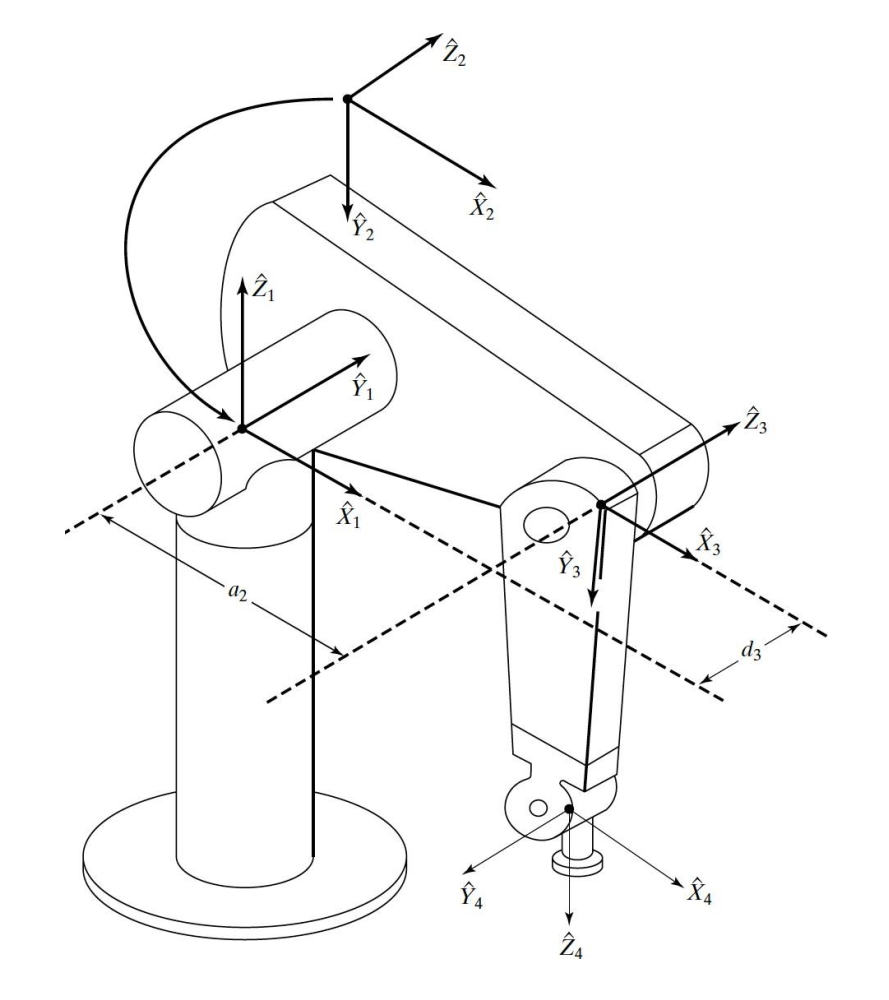
\includegraphics[width=\linewidth]{structure.png}
    \caption{PUMA560的形状示意图}
\end{figure}
\section{主要方法}
\begin{enumerate}
    \item 寻路算法

    首先我们考虑如何在位形空间中找到一条合适的路径,我们采用A*图搜索算法。

    A*算法由评价函数$f(n)=g(n)+h(n)$指导进行,其中的$g(n)$为成本函数,它代表从起点走到节点$n$所花费的实际成本;而$h(n)$则是启发函数,它用于估计从$n$节点到达种终点的成本。

    在评价函数的指导下,我们根据节点的评价函数,从小到大依次展开节点,并将展开节点的子节点加入开放列表中,从而可以让我们尽快地找到一条从起点通往终点的路线。

    在A*图搜索中,我们需要维护两个列表,一个是开放列表,一个则是封闭列表。
    
    开放列表用于记录所有可考虑选择的节点,类似于树搜索中的边缘集合,可以用优先队列实现。

    而封闭列表则记录所有不再考虑的节点,可以用来避免对同一节点的重复访问。

    A*图搜索的伪代码如图所示:

    \begin{figure}[htbp]
        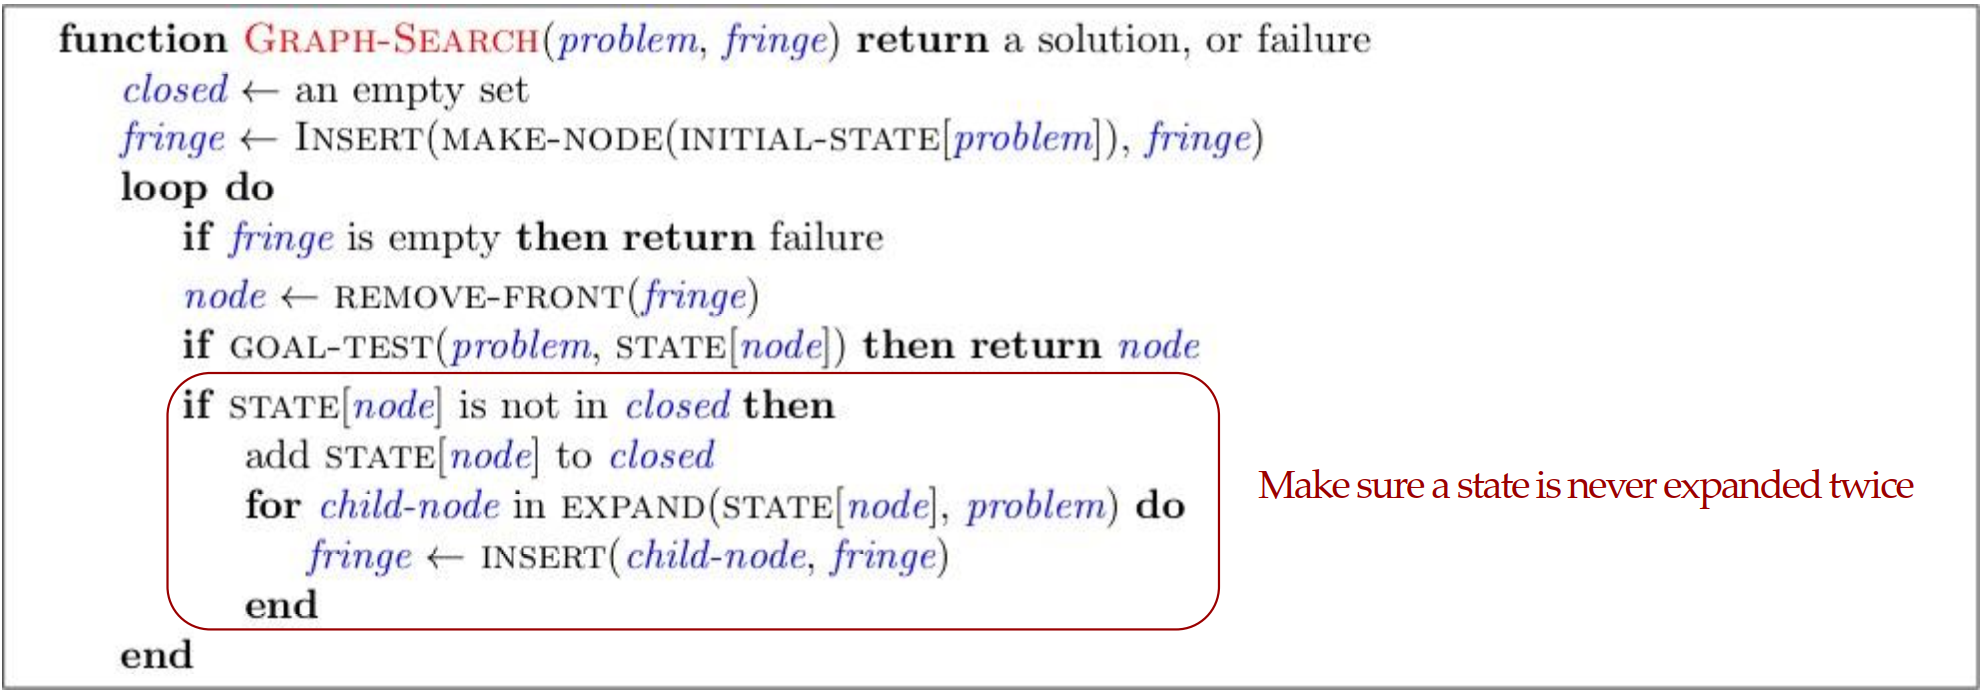
\includegraphics[width=\linewidth]{A.png}
        \caption{A*算法的伪代码}
    \end{figure}

    \item 位形规划

    之后我们来考虑对位形的规划,首先是对于重心的规划。我们假设每根机械臂单位长度的重量为1,物品的重量为$m$,平台为$2a\times 2a$,那么对于PUMA560就有方程:
    \begin{equation}
        M_0 = h_0\times(0, 0)
    \end{equation}
    \begin{equation}
        M_1 = d_3\times\frac{(d_3\cos(\theta_1), d_3\sin(\theta_1))}{2}
    \end{equation}
    \begin{equation}
        M_2 = a_2\times(d_3c_1+\frac{a_2s_1c_2}{2}, d_3s_1-\frac{a_2c_1c_2}{2})
    \end{equation}
    \begin{equation}
        M_3 = d_4\times(d_3c_1+a_2s_1c_2+\frac{d_4s_3}{2}, d_3s_1-a_2c_1c_2-\frac{d_4s_3}{2})
    \end{equation}
    \begin{equation}
        M_m = m\times(d_3c_1+a_2s_1c_2+d_4s_3, d_3s_1-a_2c_1c_2-d_4s_3)
    \end{equation}
    \begin{equation}
        (-a, -a)\leq \frac{M_0+M_1+M_2+M_3+M_m}{h_0+d_3+a_2+d_4+m}\leq (a, a)
    \end{equation}
    以上即为重心对机械臂位形的要求,这里$h_0$为基座的高度,$d_3$,$a_2$,$d_4$是三个机械臂各自的长度,$m$为物品重量对应的长度。

    其次我们考虑逆运动学,即如何根据变换矩阵得到机械臂的各个角度。在给定一个需要到达的点之后,我们需要根据逆运动学来解算出PUMA560六个角度参数的值。由于这个方程很难有解析解,我们要采用的方法是数值求解。

    数值求解的一个基本方法是牛顿法,牛顿法通过不断求导以逼近真实零点,公式如下:
    \begin{equation}
        f(x_0+\Delta)\approx f(x_0)+f'(x_0)\Delta
    \end{equation}
    根据这一个公式,我们可以得到一组数列${x_n}$,它满足迭代公式:
    \begin{equation}
        x_n = x_{n-1}-\frac{f(x_{n-1})}{f'(x_{n-1})}
    \end{equation}
    牛顿法仅适用于一元的函数,对于多元的向量函数,我们应该使用牛顿高斯法,即为了求解
    \begin{equation}
        \boldsymbol{f}(\boldsymbol{x})=\boldsymbol{0}
    \end{equation}
    给出的迭代公式为
    \begin{equation}
        \boldsymbol{x}_{n+1}=\boldsymbol{x}_n-(\boldsymbol{J_f}^\intercal\boldsymbol{J_f})^{-1}\boldsymbol{J_f}^\intercal\boldsymbol{f}(\boldsymbol{x}_n)
    \end{equation}
    这里的$\boldsymbol{J_f}$是函数$\boldsymbol{f}$的Jacobi矩阵。

    在牛顿高斯法之后,还有一个改进的版本,它通过加入可调节参数$\lambda$来使得收敛效率可调节,即Levenberge-Marquardt法:
    \begin{equation}
        \boldsymbol{x}_{n+1}=\boldsymbol{x}_n-(\boldsymbol{J_f}^\intercal\boldsymbol{J_f}+\lambda\boldsymbol{I})^{-1}\boldsymbol{J_f}^\intercal\boldsymbol{f}(\boldsymbol{x}_n)
    \end{equation}

    Levenberge-Marquardt法能提供数非线性最小化(局部最小)的数值解。此算法能借由执行时修改参数达到结合高斯-牛顿算法以及梯度下降法的优点,并对两者之不足作改善(比如高斯-牛顿算法之反矩阵不存在或是初始值离局部极小值太远)

    最后,我们来考虑三维空间对机械臂运动的约束。注意到不论何种宽度的道路,机械臂都可以通过在竖直方向完全伸直来侧向通过这一条道路,且这种情况不会影响机械臂的物理平衡条件,因为倘若在这种情况下都无法做到物理平衡,则其他位形也必然不能,证明如下:

    我们假设一个搭载了物体的机械臂在竖直方向完全伸直之后仍然无法达到平衡状态,这就意味着在第一条机械臂,即坐标轴$Y_1$方向无法平衡。然而,无论如何怎么改变第二条机械臂与第三条机械臂的角度,都无法减少在$Y_1$方向上的重量,因此这种构型必然失去平衡。

    因此,我们只需要知道,为了达到物理平衡,机械臂至少需要达到的最低高度为多少,即“天花板的高度”,这将是三维空间中唯一限制机械臂自由运动的因素。
\end{enumerate}
\section{实验结果}
在这一部分中,我们将介绍我们所做的模拟结果,包括两个部分,第一个是实验环境搭建,第二个是实验结果。
\begin{enumerate}
    \item 实验环境搭建
    
    我们采用的模拟程序是用的python中的roboticstoolbox库,这个库为设计、仿真、测试和部署操作臂与移动机器人应用提供了工具与算法。
    对于操作臂,该工具箱包含了使用刚体树表示形式的碰撞检测、路径规划、轨迹生成、正向和反向运动学以及动力学的算法。
    对于移动机器人,该工具箱提供了用于映射、定位、路径规划、路径跟随和移动控制的算法。

    在我们这次的实验中,主要用到的是roboticstoolbox中提供的LM逆运动学算法,它可以把需要到达的位置转换为我们的变换矩阵,以及对应的六个角度。

    在表达变换矩阵的时候,我们采用的是spatialmath库中的pose3d,他能用于记录各种三维变换矩阵。

    在可视化过程中,我们使用了matplotlib与robotictoolbox两个库,它可以模拟出来对应的简化机械臂形态,让我们能更好的判断程序是否能够正常运行。

    在代码里面,我们首先检测物品的高度,来判断是否是可以到达的高度,如果整个机械臂伸直都无法到达物品的高度,我们则直接认为该问题无解。

    之后,我们检测物品的重量,看看是否存在一种能保持平衡的位形,如果不存在,那么这个问题也无解。

    再然后,我们考虑是否存在一种平衡位形能够让机械臂能够到起点和终点,如果不行,那么机械臂将无法完成物体的搬运。与此同时,我们还需要检查这两种位形的高度是否抵达了限高,如果超过了限高,这个问题同样无解。

    最后,我们通过A*算法规划从起点到终点的路径,并将它应用到机械臂的运动上。

    \item 实验结果
    
    模拟的结果如图所示,图3是PUMA560初始的位置

    \begin{figure}[htbp]
        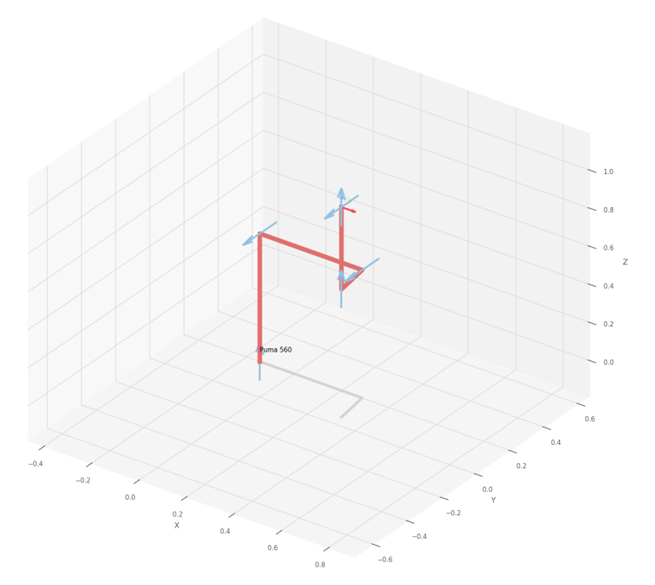
\includegraphics[width=\linewidth]{init.png}
        \caption{PUMA560的初始位置}
    \end{figure}

    我们输入一组坐标,能看到机械臂抓取物体的位形如图4所示

    \begin{figure}[htbp]
        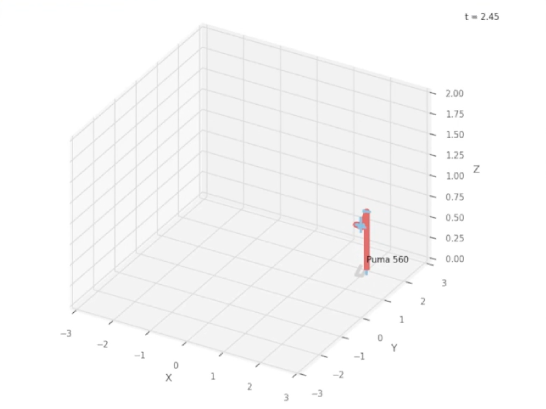
\includegraphics[width=\linewidth]{start.png}
        \caption{PUMA560的抓取位置}
    \end{figure}

    之后机械臂放置物体的位形如图5所示

    \begin{figure}[htbp]
        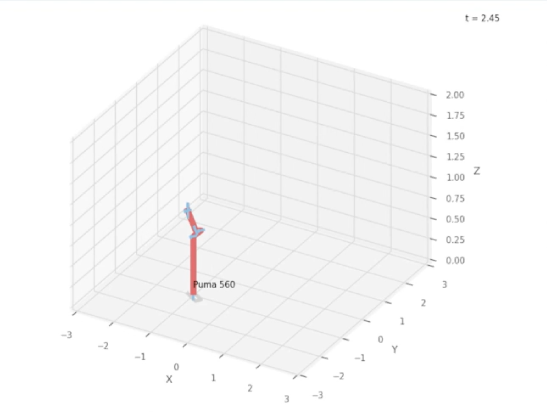
\includegraphics[width=\linewidth]{goal.png}
        \caption{PUMA560的放置位置}
    \end{figure}

    在规划的过程中,我们判断了机械臂的位形的平衡条件,保证了在任一时刻机械臂都处于平衡状态,从而也有实际运用的意义。

    与此同时,我们也考虑了限高的要求,能够满足三维空间的约束。
\end{enumerate}

\section{结论}
在这个实验中,我们建立了一个模拟机械臂运动的环境,为机械臂运动规划与运动的平衡性提出了一定的理论支撑,同时我们在实验中模拟了真实情况下的机械臂运动,试图最优化了机械臂运动的成本。
诚然,这个实验依然存在一定的缺陷,例如只考虑了PUMA560这一种机械臂的构型,而没有把整个方法推广到所有机械臂中去,又比如只考虑了在平面上的运动,而不是真实场景中更常见的崎岖不平的表面中的运动。
未来的工作还可以考虑如何优化机械臂的旋转方式,使其转过的角度最小,或者是在机械臂平移的同时保持平衡且转动机械臂,来节省搬运的时间。
\begin{thebibliography}{00}
\bibitem{b1} Lourakis M I A. A brief description of the Levenberg-Marquardt algorithm implemented by levmar[J]. Foundation of Research and Technology, 2005, 4(1): 1-6.
\bibitem{b2} Armstrong B, Khatib O, Burdick J. The explicit dynamic model and inertial parameters of the PUMA 560 arm[C]//Proceedings. 1986 IEEE international conference on robotics and automation. IEEE, 1986, 3: 510-518.
\bibitem{b3} Piltan F, Emamzadeh S, Hivand Z, et al. PUMA-560 robot manipulator position sliding mode control methods using MATLAB/SIMULINK and their integration into graduate/undergraduate nonlinear control, robotics and MATLAB courses[J]. International Journal of Robotics and Automation, 2012, 3(3): 106-150.
\bibitem{b4} https://pypi.org/project/roboticstoolbox-python/0.10.1/
\bibitem{b5} https://pypi.org/project/spatialmath-python/
\end{thebibliography}

\end{document}
